En los resultados tenemos que, para el primer enfoque, los tiempos con programación dinámica son muy bajos comparados con fuerza bruta, y del gráfico podemos ver que la eliminación fue el que mas se tardo, esto se atribuye a que para que solo sea una eliminación, hay que tener 1 carácter de mas en palabra, lo cual hace que su longitud sea mas larga, teniendo asi mas casos de prueba, por otro lado tenemos que sustituir es el que menos tarda, y esto se debe a que como las palabras son muy similares, después de sustituir, todo sera igual, no haciendo asi, mas llamadas recursivas.



\begin{figure}[H]
    \centering
    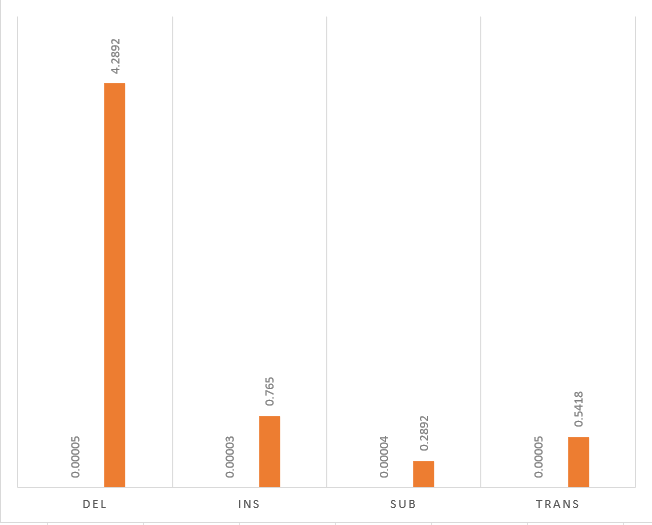
\includegraphics[width=10cm, height=8cm]{images/especifico.png}
    \caption{Gráfico para funciones especificas}
    \label{fig:especifico}
\end{figure}

Con el segundo enfoque se obtiene que al igual que en enfoque anterior, pero en este se puede presenciar de mejor manera como crece exponencialmente el enfoque de fuerza bruta, y como programación dinámica crece mínimamente, por otro lado el espacio se mantiene constante, en general fuerza bruta utilizo menos espacio que programación dinámica, que es lo que se esperaba en un inicio, sin embargo a aveces resultaba dar distintos espacios para una misma entrada, esto se debe a que el sistema operativo busca la mejor manera de manejar la memoria dinámica (Heap)

\begin{figure}[H]
    \centering
    \begin{minipage}[t]{0.5\textwidth}
        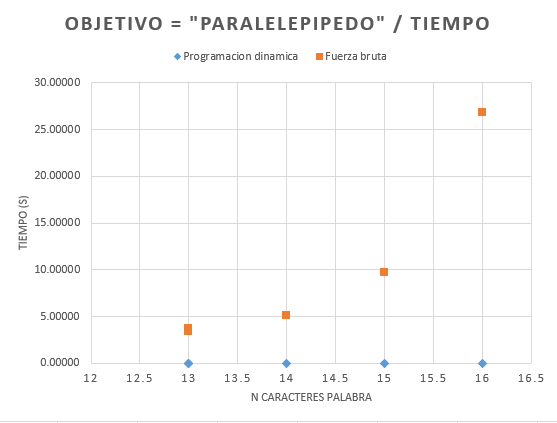
\includegraphics[width=\textwidth]{images/palabras-generadasT.png}
    \end{minipage}%
    \begin{minipage}[t]{0.5\textwidth}
        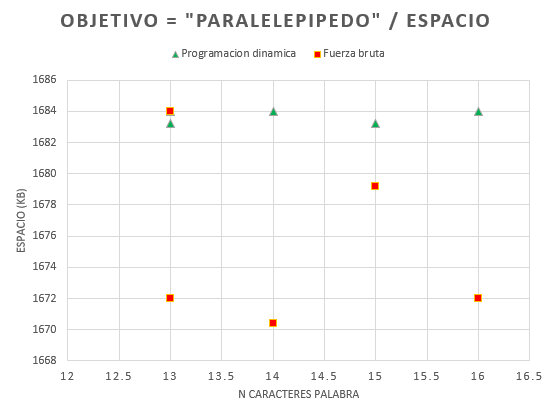
\includegraphics[width=\textwidth]{images/palabras-generadasE.png}    \end{minipage}%
    \caption{Gráficos con palabras aleatorias para objetivo paralelepipedo}
    \label{fig:random}
\end{figure} 

Ahora para los siguientes gráficos se combinaran los enfoques para comparar de la forma mas rigurosa posible, con los enfoques donde la palabra crece se genero el siguiente gráfico para programación dinámica y fuerza bruta:

\begin{figure}[H]
    \centering
    \begin{minipage}[t]{0.5\textwidth}
        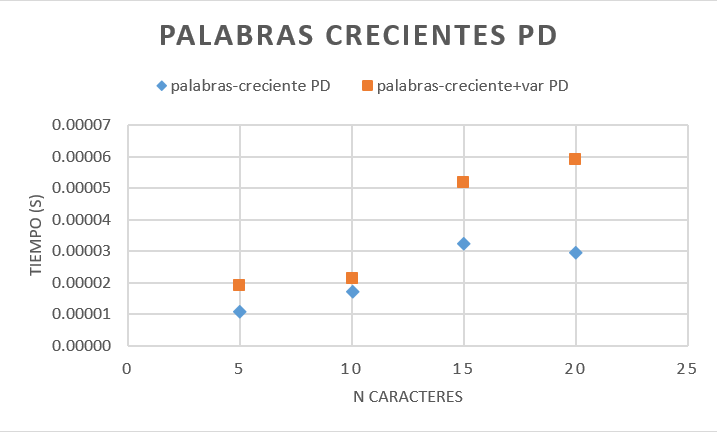
\includegraphics[width=\textwidth]{images/palabras-credientes-pd.png}
    \end{minipage}%
    \begin{minipage}[t]{0.5\textwidth}
        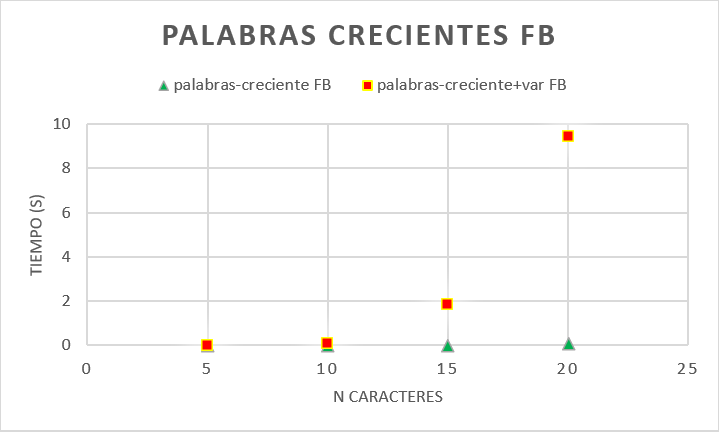
\includegraphics[width=\textwidth]{images/palabras-credientes-fb.png}    \end{minipage}%
    \caption{Gráficos para palabras de largo creciente con objetivo fijo}
    \label{fig:Pcreciente}
\end{figure} 

Estos gráficos se separaron para que sea mas facil ver como crece programacion dinamica, que antes parecia ser constante, aqui se revela que no lo es, se comporta de forma mas lineal, aunque el grafico no es muy exacto porque las palabras para ir aumentando tienen que cambiar.\\
también se observa que si los caracteres son poco variados, el programa funcionara mejor con cualquiera de los enfoques, de hecho para fuerza bruta, si los caracteres son variados se comporta mucho mas exponencial que si no lo son, esto se debe a que es mas probable que en algún momento se encuentre algún carácter igual,  reduciendo las llamadas recursivas, y por tanto reduciendo los tiempos.\\
Por otro lado se ve la gran diferencia que hay entre fuerza bruta y programación dinámica, esta esta a una escala mucho menor, sus mayor valor no alcanzan a ser 0.001 segundos, mientras que con fuerza bruta, para palabras de 15 caracteres ya tarda 2 segundos.\\


Los siguientes gráficos muestran como se comportan los tiempos cuando palabra y objetivo tienen el mismo largo y este va variando, aqui ya se pierde mucho la exactitud porque palabra y objetivo tienen que ir cambiando para aumentar su tamaño, lo cual hace que los problemas sean distintos.

\begin{figure}[H]
    \centering
    \begin{minipage}[t]{0.5\textwidth}
        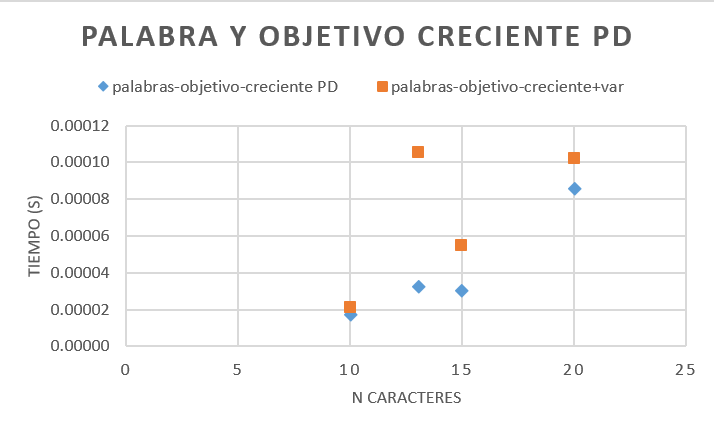
\includegraphics[width=\textwidth]{images/po-credientes-pd.png}
    \end{minipage}%
    \begin{minipage}[t]{0.5\textwidth}
        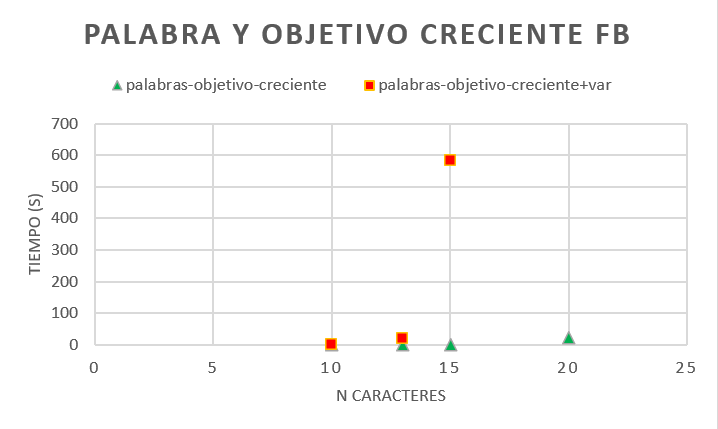
\includegraphics[width=\textwidth]{images/po-credientes-fb.png}    \end{minipage}%
    \caption{Gráficos para palabras y objetivos de largo creciente}
    \label{fig:POcreciente}
\end{figure} 

